\documentclass[dvipdfmx,autodetect-engine,titlepage]{jsarticle}
\usepackage[dvipdfm]{graphicx}
\usepackage{ascmac}
\usepackage{fancybox}
\usepackage{listings}
\usepackage{plistings}
\usepackage{itembkbx}
\usepackage{amsmath}
\usepackage{svg}
\usepackage{url}
\usepackage{graphics}
\usepackage{listings,jvlisting}

\textheight=23cm
\renewcommand{\figurename}{図}
\renewcommand{\tablename}{表}
\newenvironment{code}
{\vspace{0.5zw}\VerbatimEnvironment  
\begin{screen} 
\baselineskip=1.0\normalbaselineskip
 \begin{Verbatim}}
{\end{Verbatim}
\baselineskip=\normalbaselineskip
 \end{screen}\vspace{0.5zw}} 

\title{情報理工学部 SNコース 3回\\
自然言語処理第6回講義レポート\\}
\author{2600200443-6\\Yamashita Kyohei\\山下 恭平}
\date{May 20 2022}

\begin{document}

\maketitle

\section{解答}
与えられた問題についてCKY法を用いたところ、以下の3つの句構造が得られた。

\subsection{結果1}

\begin{figure}[h]
  \centering
  \begin{minipage}[b]{0.45\linewidth}
  \begin{center}
    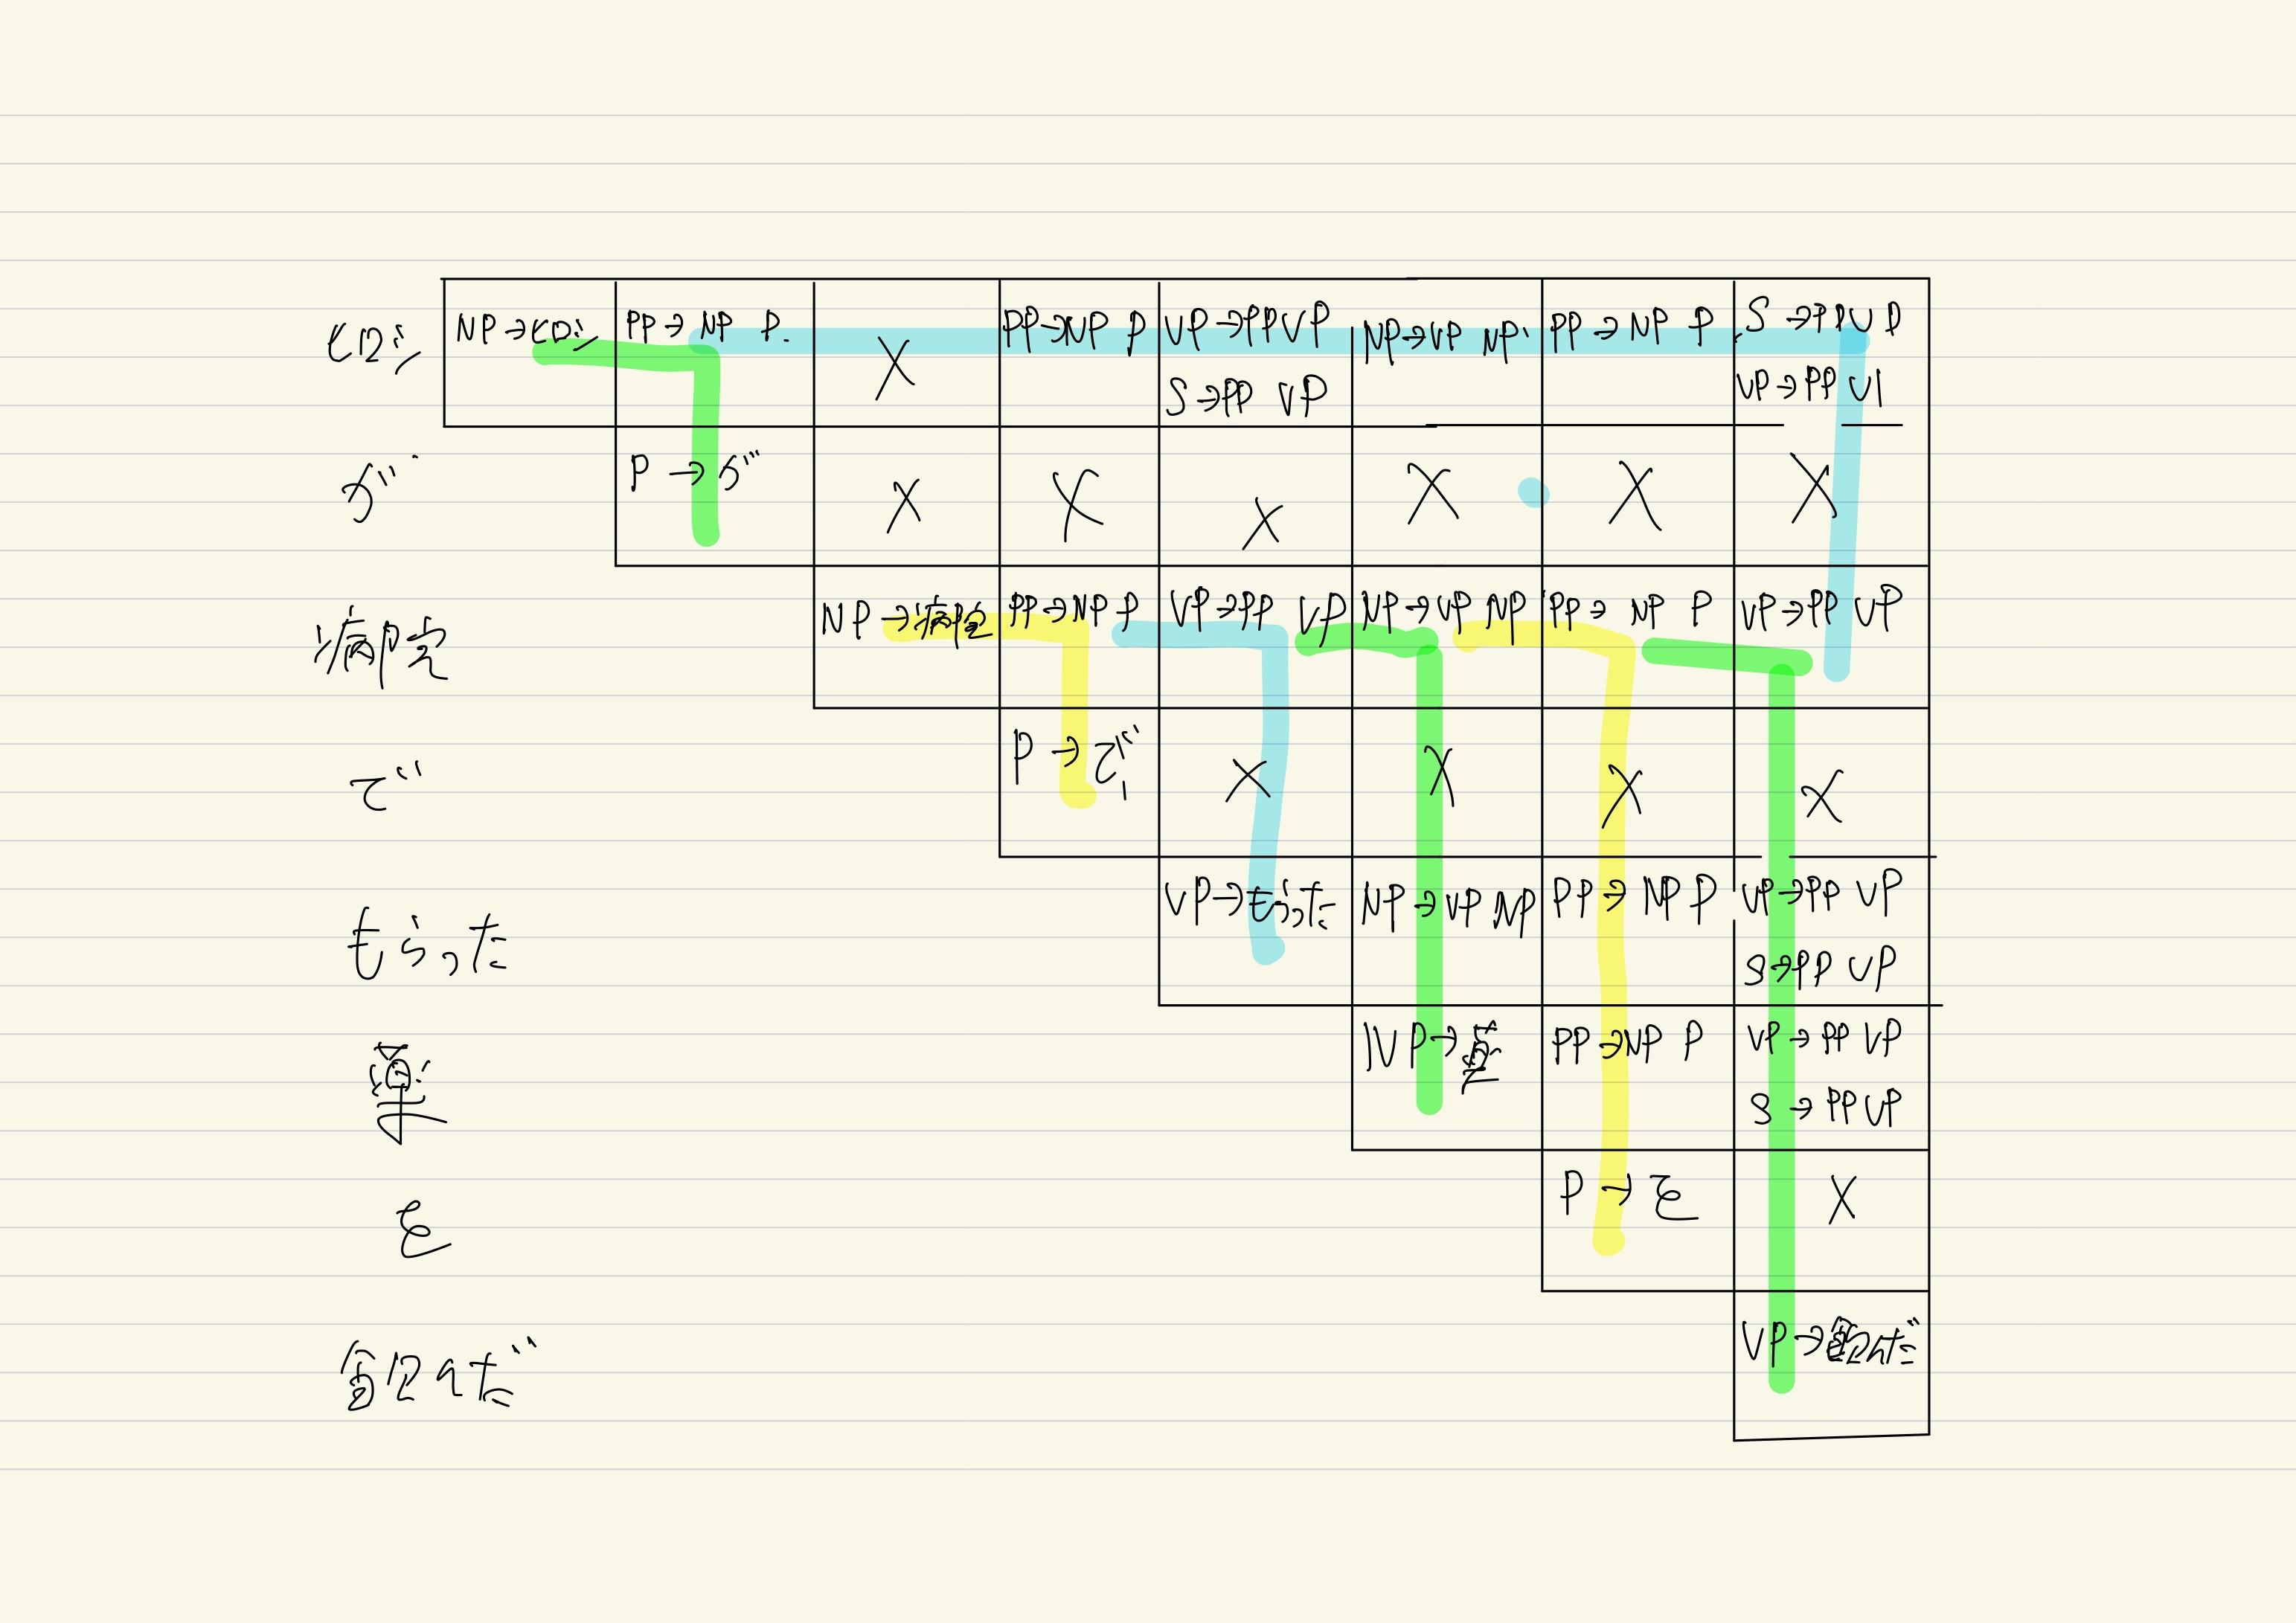
\includegraphics[keepaspectratio,scale=0.08]{pic1.jpg}
    \end{center}
    \caption{}
  \end{minipage}
  \begin{minipage}[b]{0.45\linewidth}
  \begin{center}
    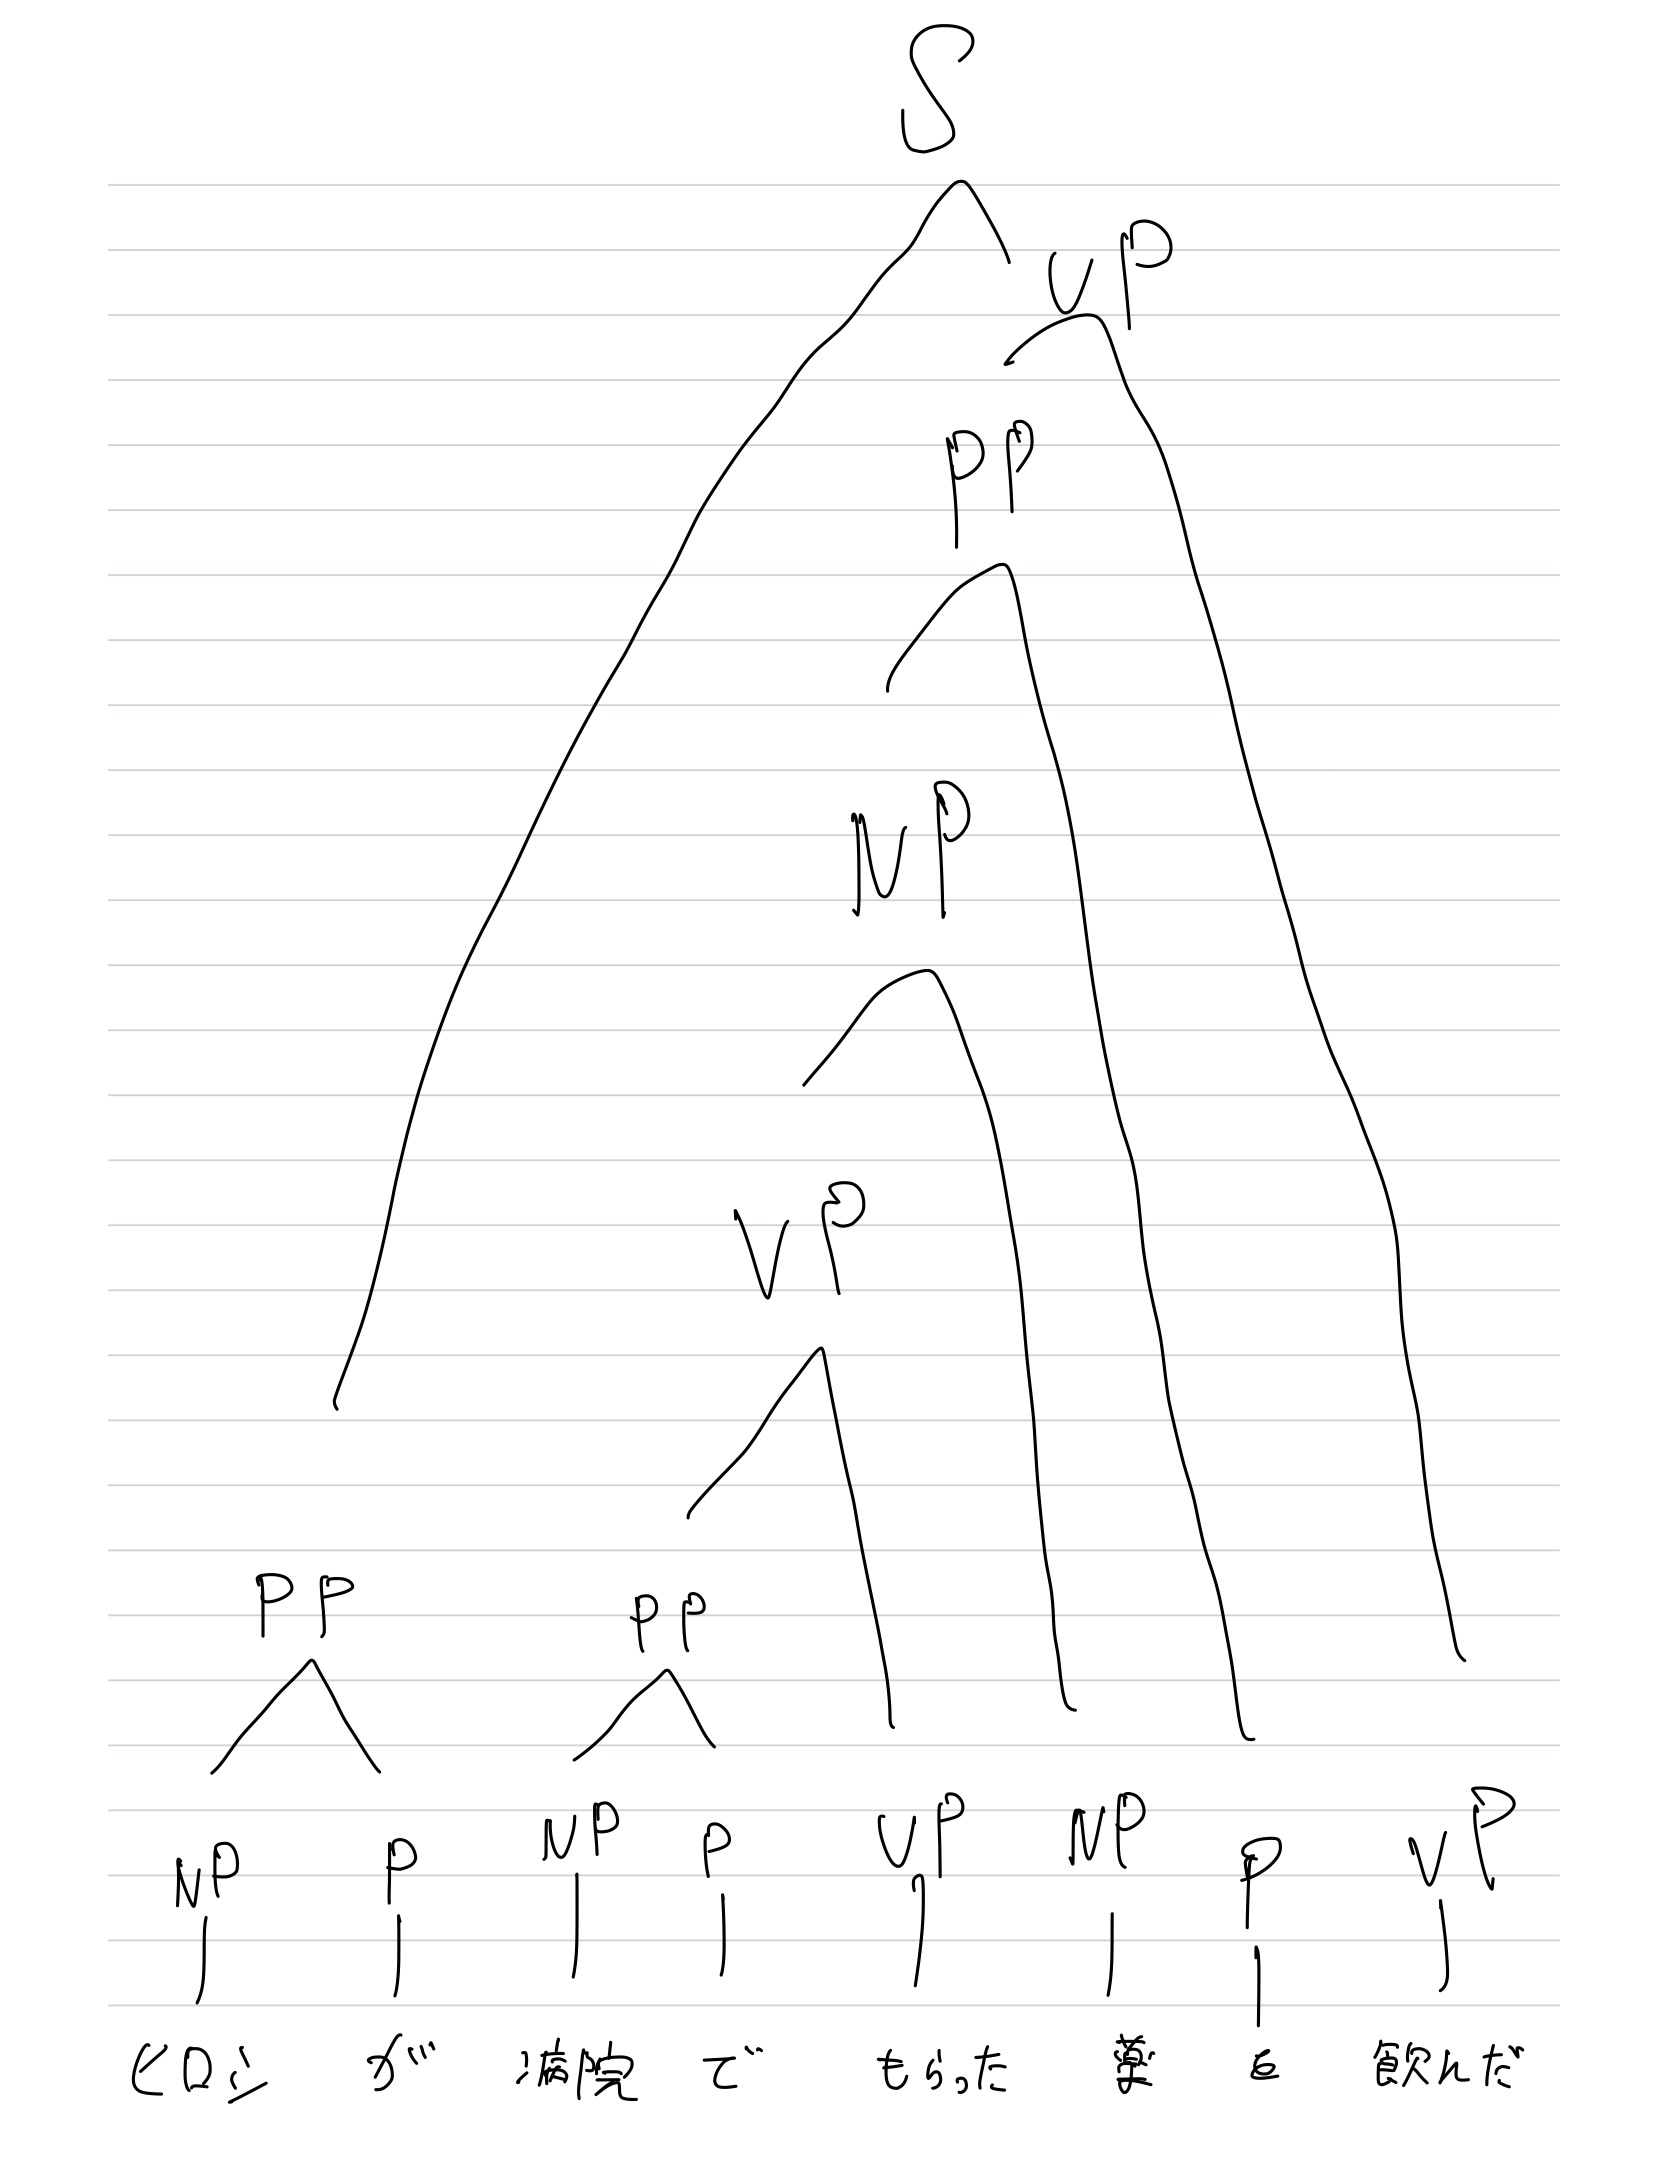
\includegraphics[keepaspectratio,scale=0.08]{pic2.jpg}
    \end{center}
    \caption{}
  \end{minipage}
\end{figure}

\subsection{結果2}

\begin{figure}[h]
  \centering
  \begin{minipage}[b]{0.45\linewidth}
  \begin{center}
    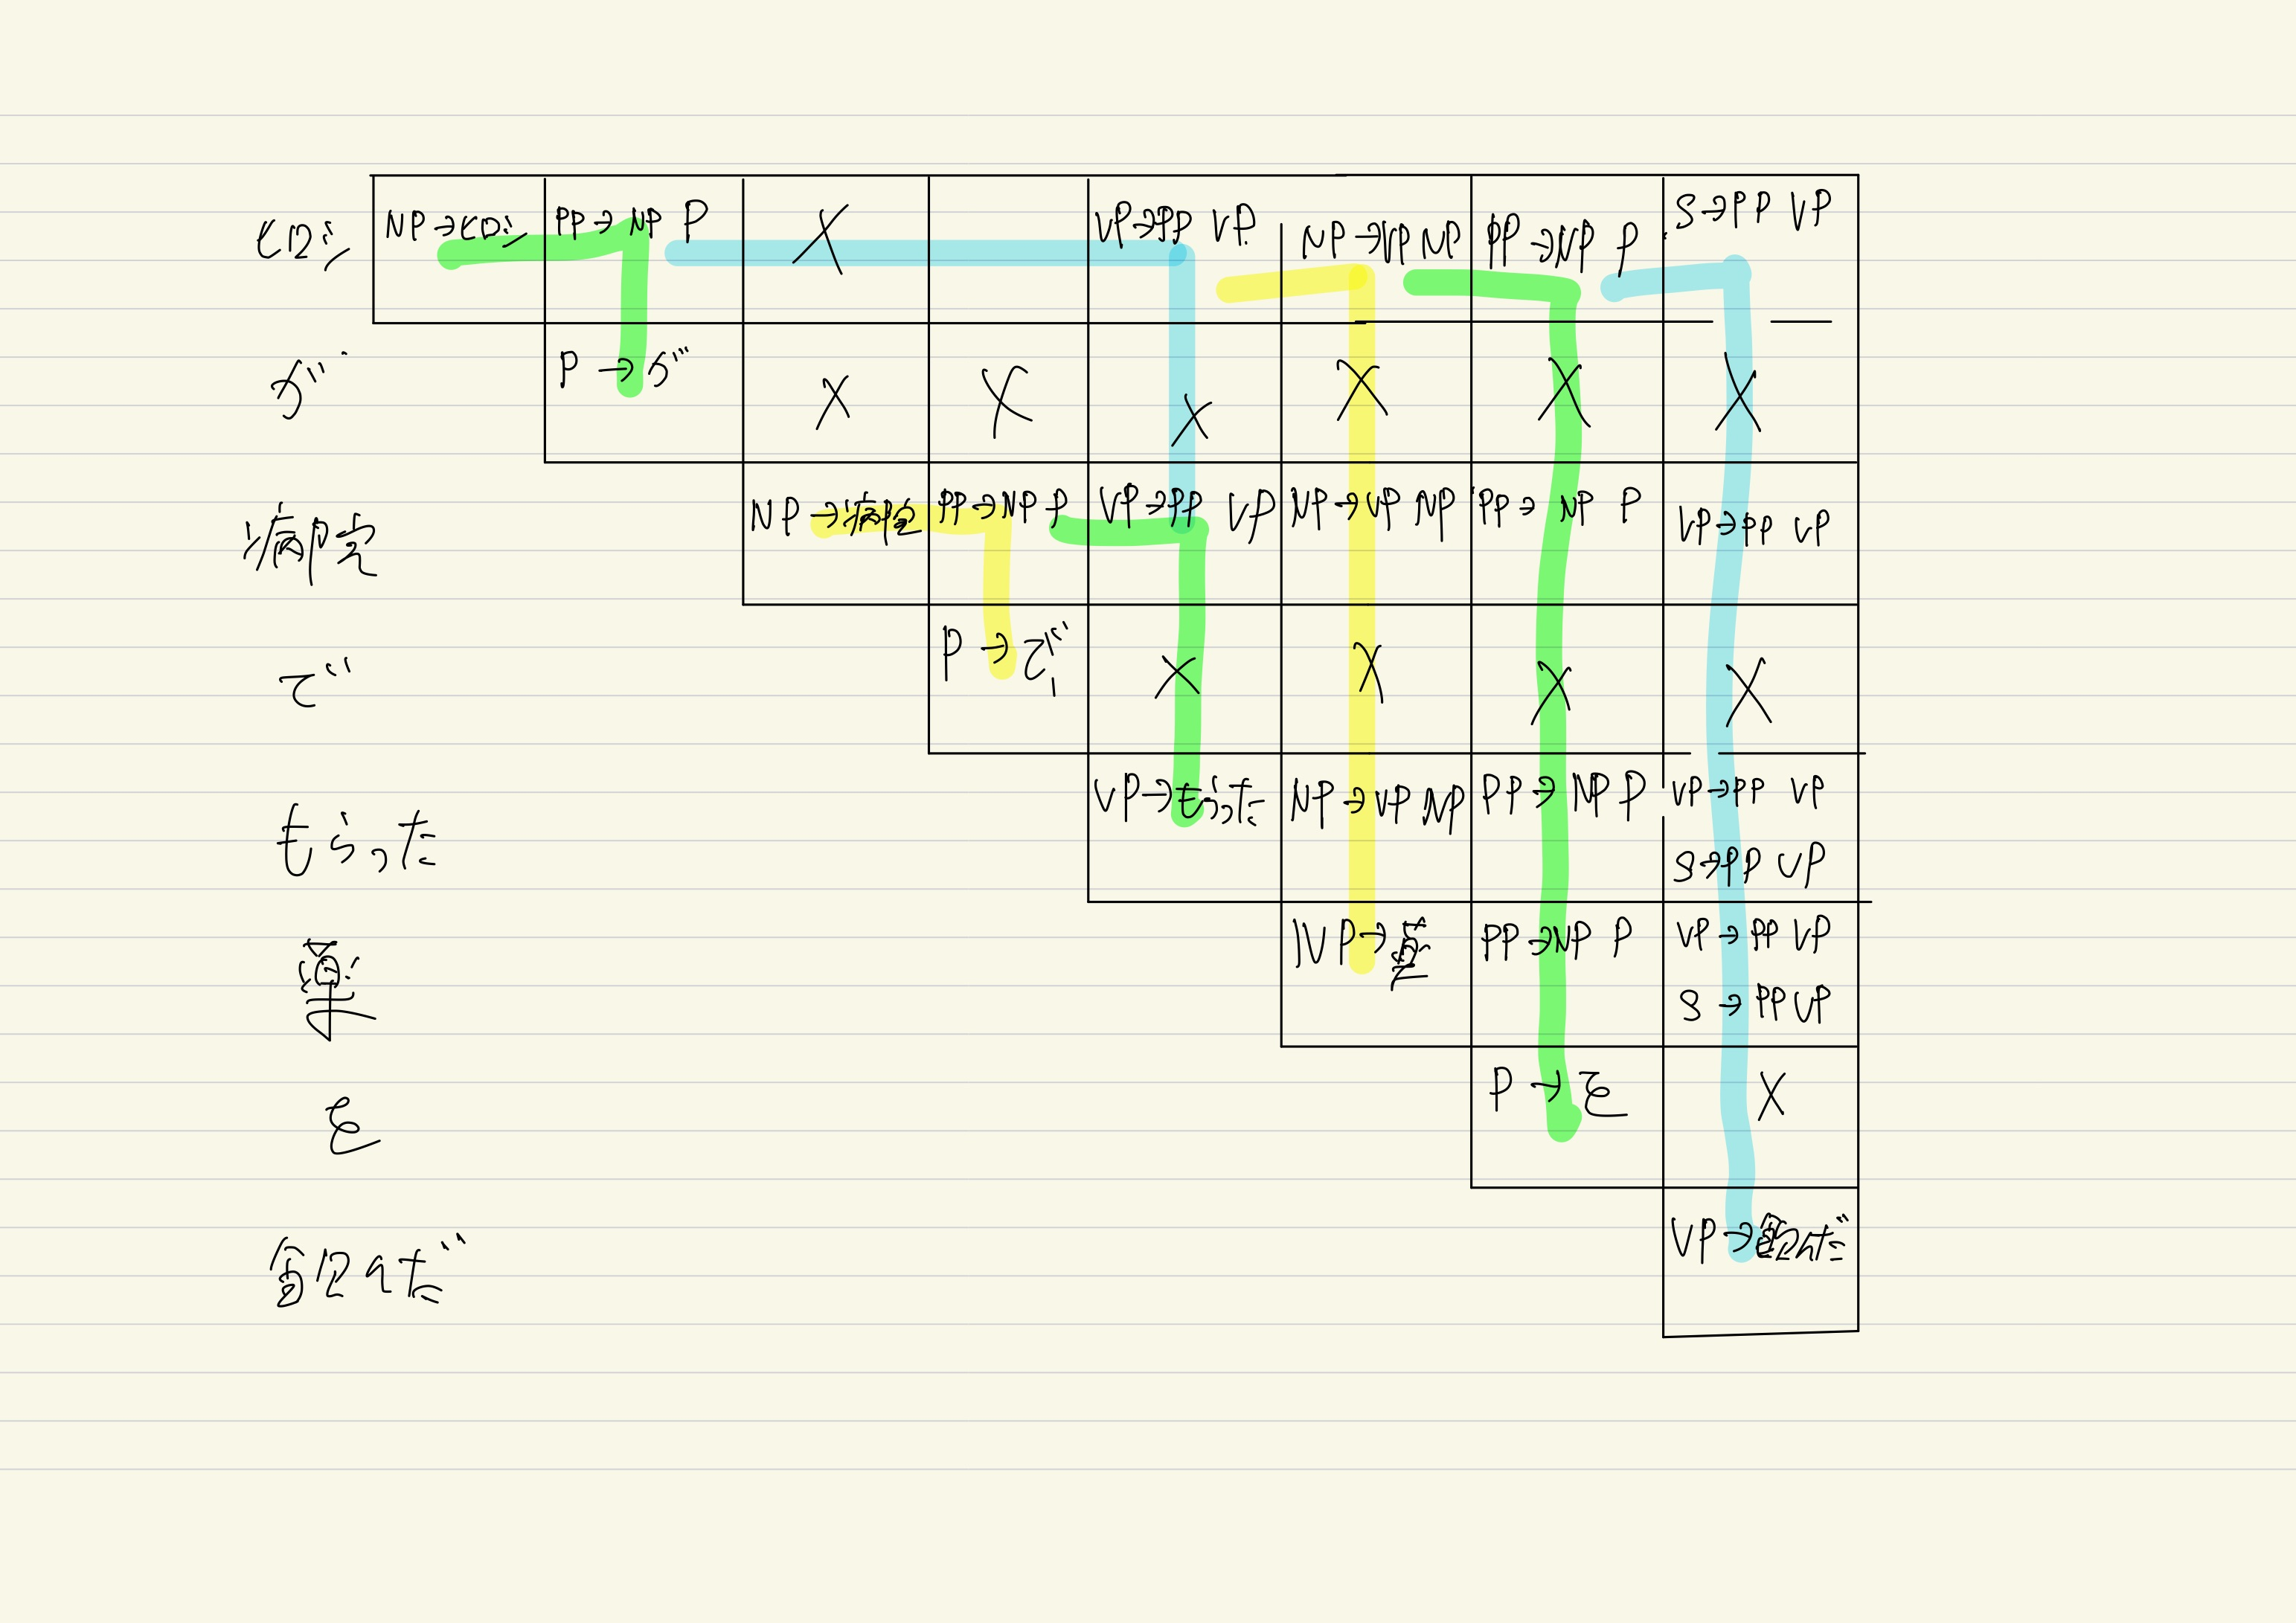
\includegraphics[keepaspectratio,scale=0.08]{pic3.jpg}
    \end{center}
    \caption{}
  \end{minipage}
  \begin{minipage}[b]{0.45\linewidth}
  \begin{center}
    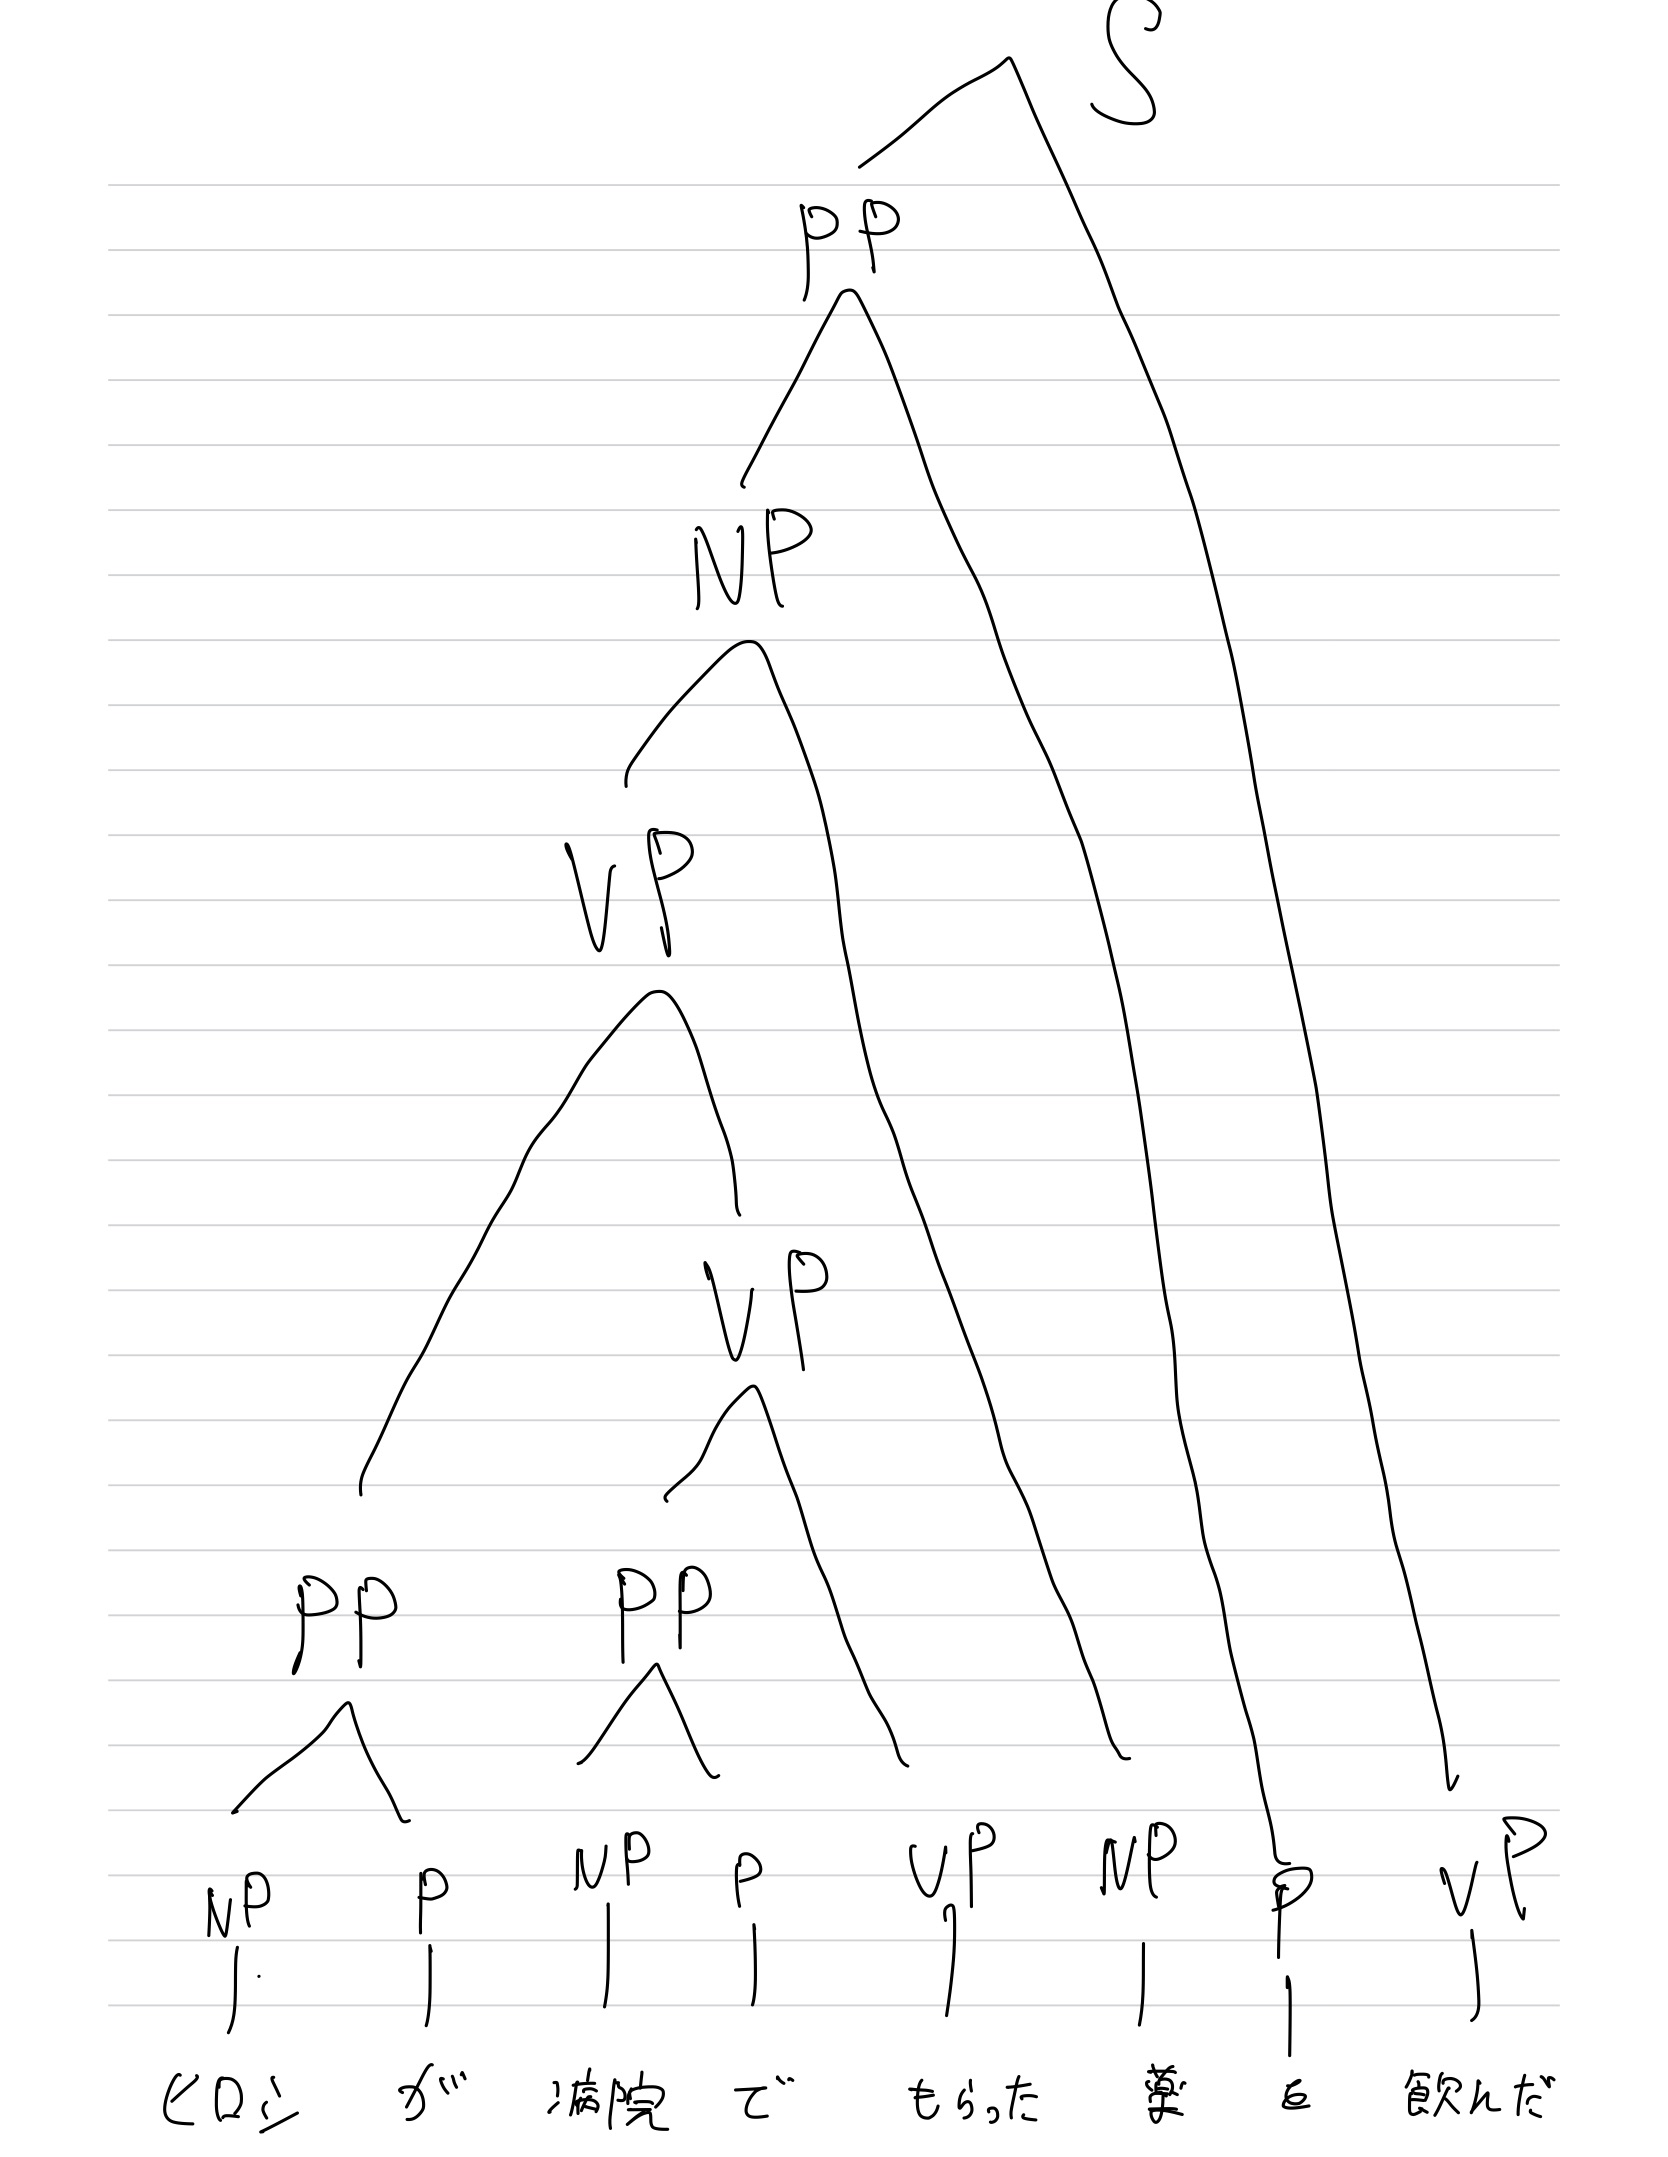
\includegraphics[keepaspectratio,scale=0.08]{pic4.jpg}
    \end{center}
    \caption{}
  \end{minipage}
\end{figure}
\newpage


\subsection{結果3}

\begin{figure}[h]
  \centering
  \begin{minipage}[b]{0.45\linewidth}
  \begin{center}
    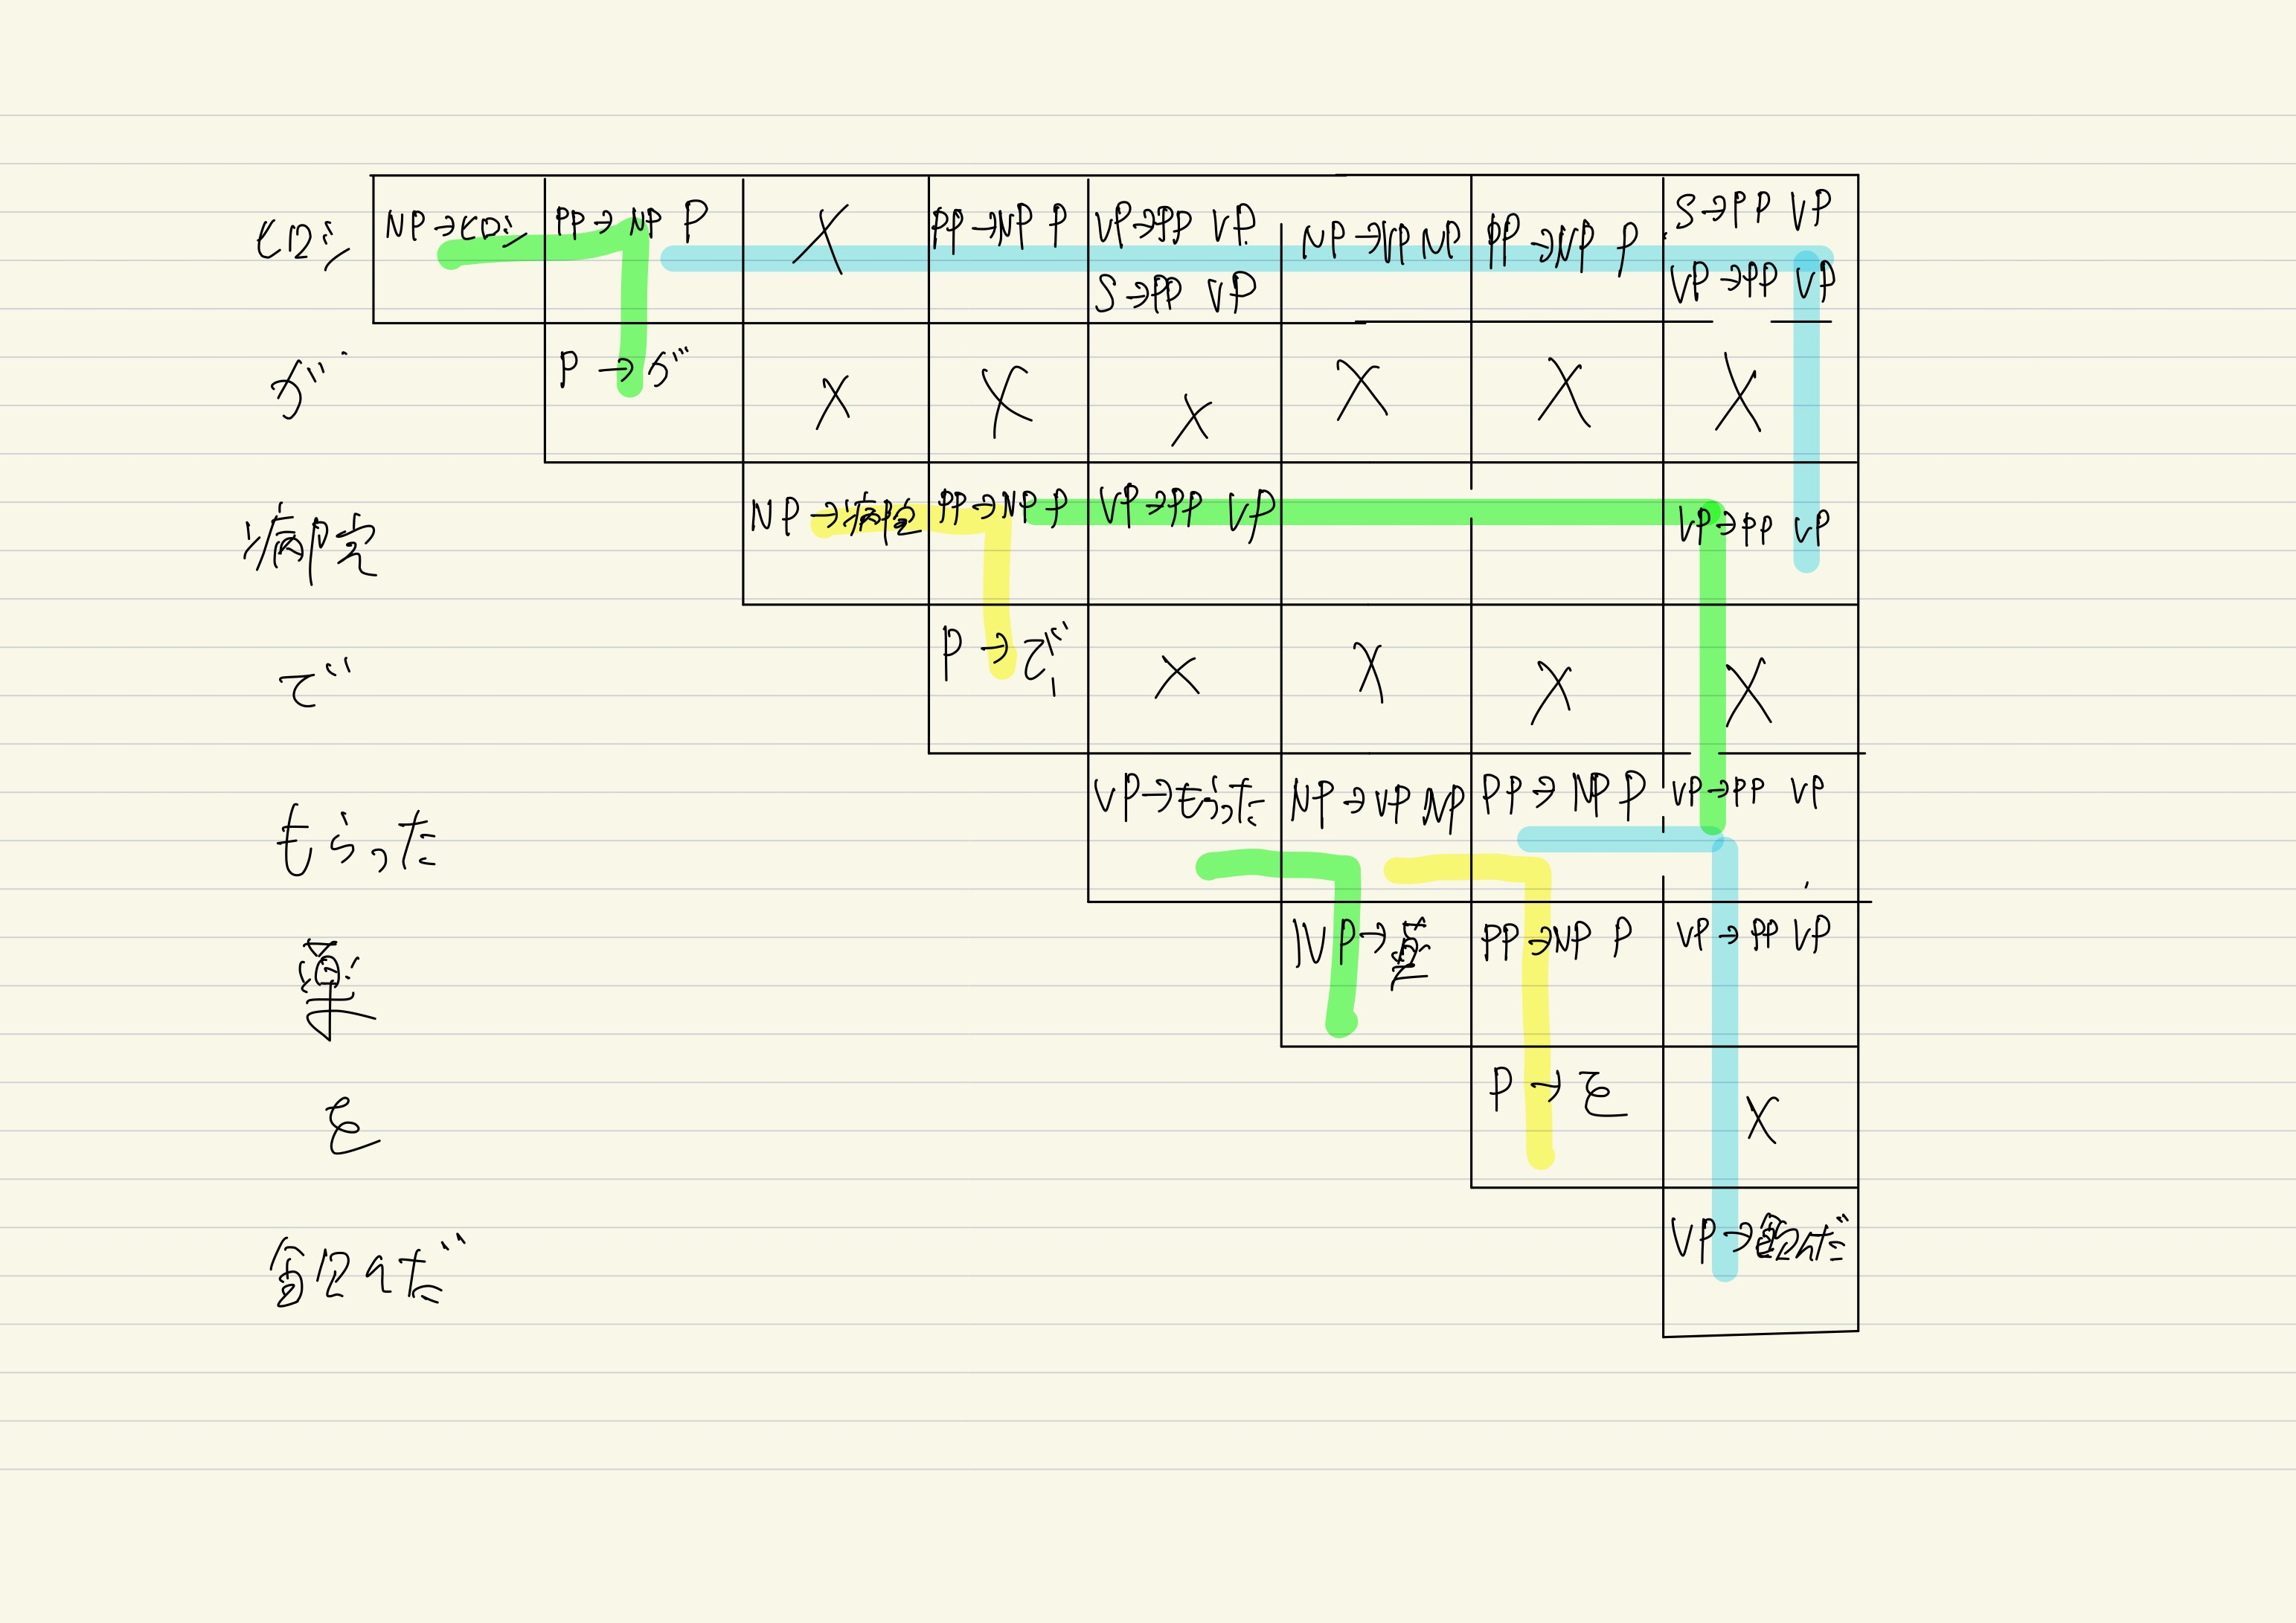
\includegraphics[keepaspectratio,scale=0.08]{pic5.jpg}
    \end{center}
    \caption{}
  \end{minipage}
  \begin{minipage}[b]{0.45\linewidth}
  \begin{center}
    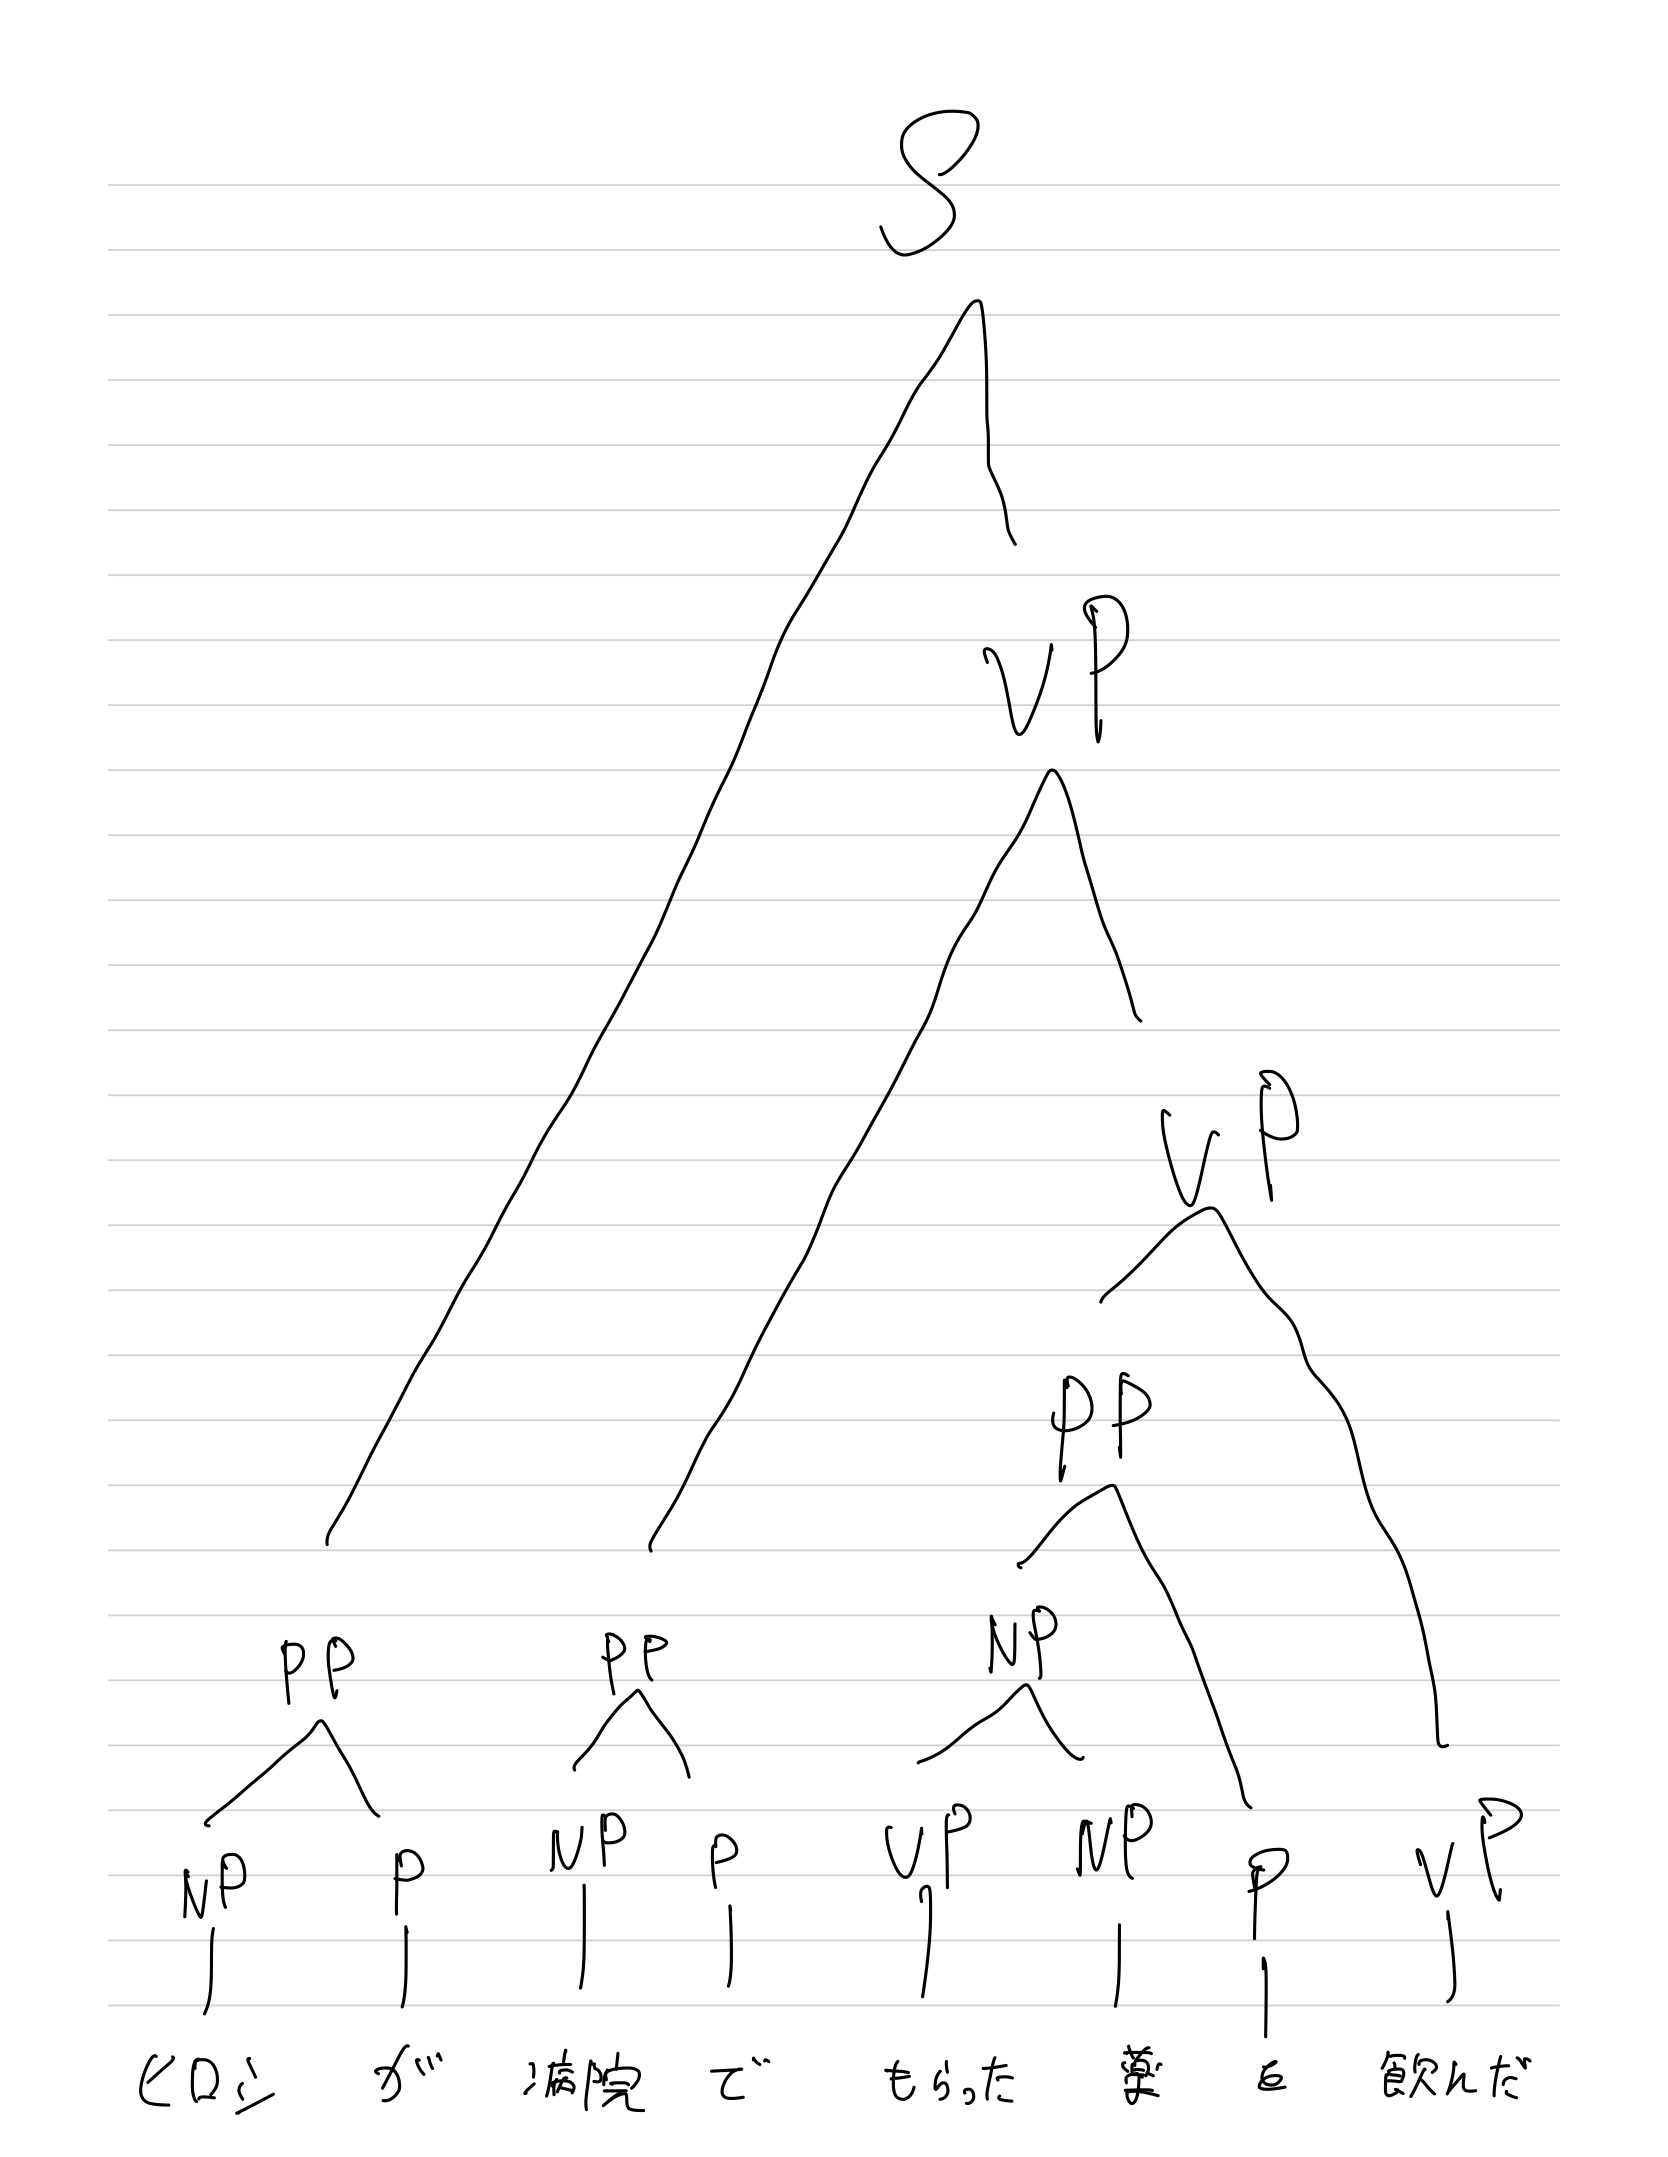
\includegraphics[keepaspectratio,scale=0.08]{pic6.jpg}
    \end{center}
    \caption{}
  \end{minipage}
\end{figure}




\end{document}

